\documentclass{article}
\usepackage{ctex}
\usepackage{xltxtra}
\usepackage{graphicx}
\usepackage{xcolor}
\usepackage{amsmath}
\usepackage{subfigure}
\usepackage{geometry}
\usepackage{amssymb}
\geometry{a4paper,left=2cm,right=2cm,top=2cm,bottom=2cm}
\graphicspath{{../fig/}}

\title{{\bf Project1: 二维Possion方程求解器}}
\author{陈震翔\\3210103924 信息与计算科学}

\date{}

\begin{document}

\maketitle

\section{理论分析}
\subsection{离散差分格式}
\subsubsection{内部格点}
对于Regular区域以及采用Nuemann边界条件的Irregular边界附近的$eqution-discretization\ points$直接采用五点差分格式,如下图的$A$和$P$:
$$L_hU_A:=\frac{4U_A-U_P-U_D-U_B-U_C}{h^2}$$
$$L_hU_P:=\frac{4U_P-U_S-U_A-U_W-U_S}{h^2}$$
\begin{figure}[h]
    \centering
    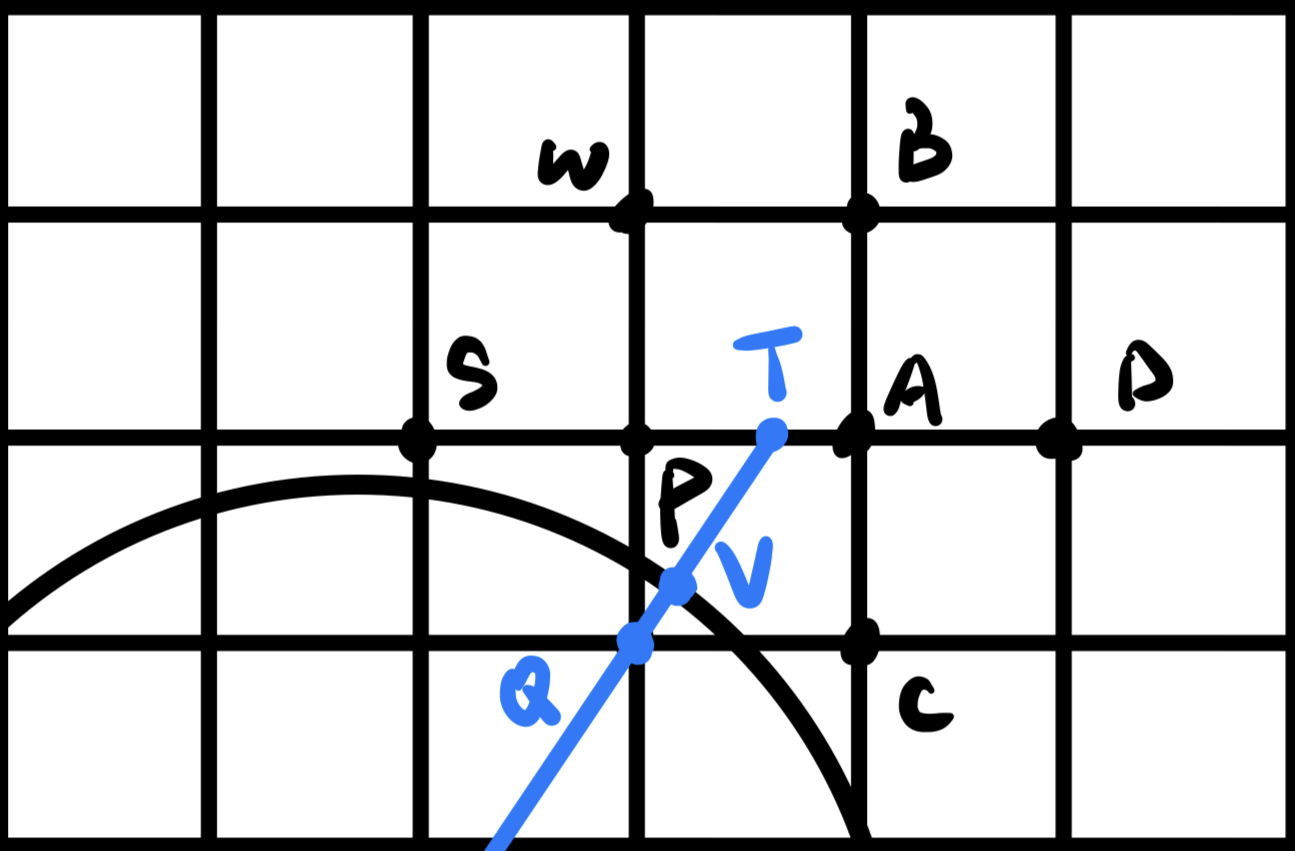
\includegraphics[width=0.5\linewidth]{discrete1.PNG}
\end{figure}

但是由图可见$P$会向圆内延拓一个点$Q$,则我们需要用到Nuemann边界条件将点$Q$纳入离散方程,首先过$Q$做边界法线方向的射线交边界于$V$,交网格于$T$,用$A$和$P$的信息对$T$进行插值得
$$U_T=\frac{|TA|}{h}U_P+\frac{|PT|}{h}U_A$$
用$T$和$Q$去近似$V$点的法向导数信息
$$\frac{U_Q-U_T}{|QT|}=g(V)$$
就得到了一条和$Q$点相关并且没有再引入额外的Irregular点的方程\\
在下面的数值实验中将会验证这是一阶精度的近似

\newpage
而对于Dirichlet边界条件附近的Irregular点,采用讲义中的Example 7.61的方式进行离散
$$L_hU_P=\frac{(1+\alpha)U_P-U_A-\alpha U_S}{\frac{1}{2}\alpha(1+\alpha)h^2}+\frac{(1+\theta)U_P-U_B-\theta U_W}{\frac{1}{2}\theta(1+\theta)h^2}$$
\begin{figure}[h]
    \centering
    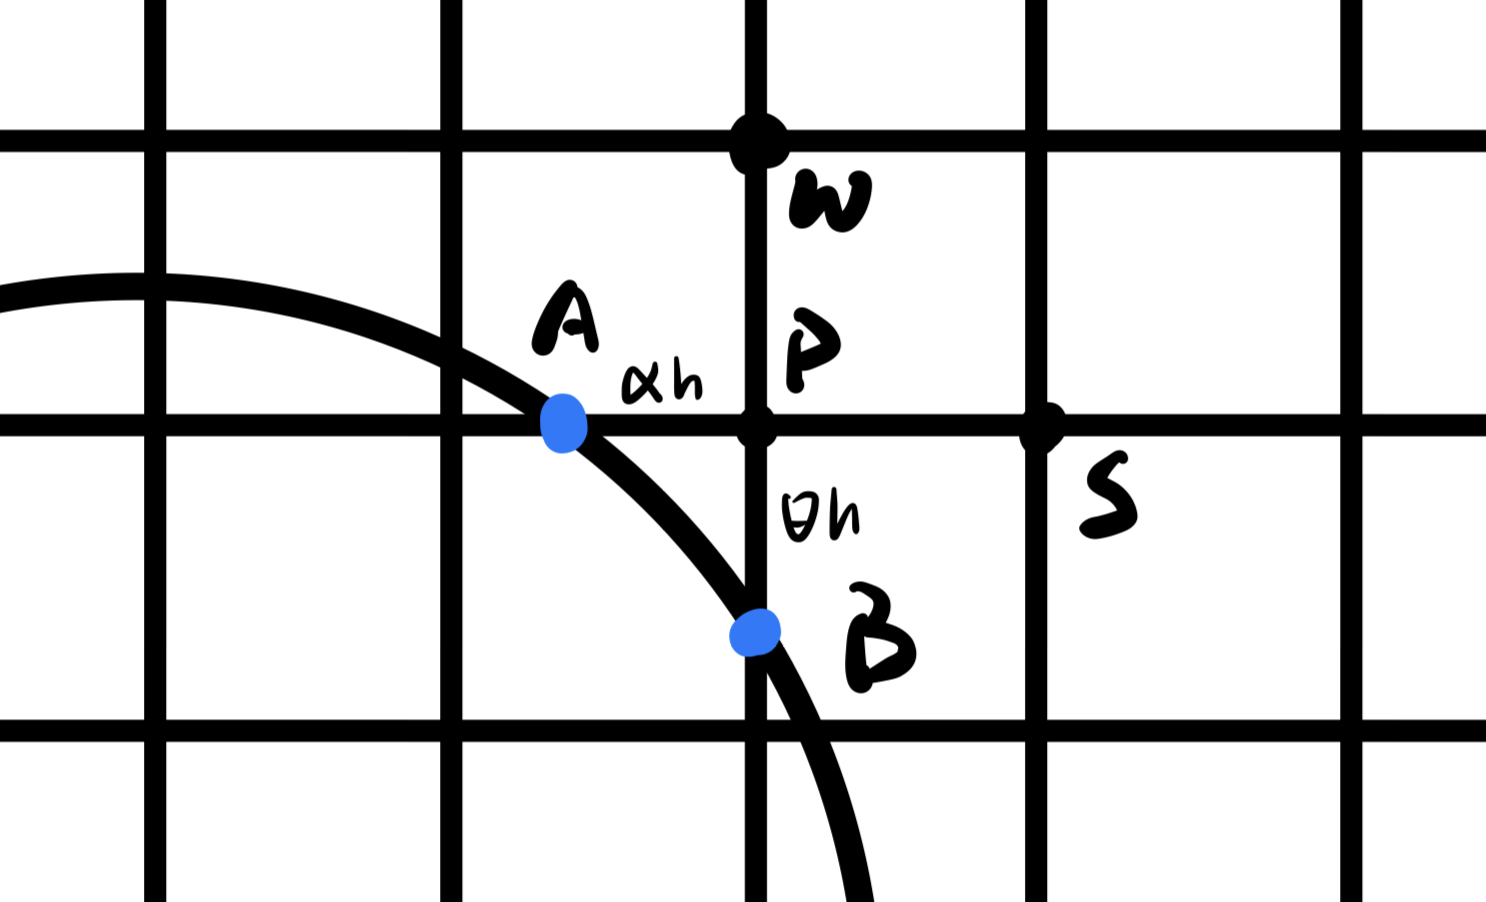
\includegraphics[width=0.5\linewidth]{discrete2.PNG}
\end{figure}

\subsubsection{边界点}
\begin{itemize}
    \item Dirichlet条件,直接给边界点赋值
    \item Nuemann条件,设$-\Delta u(P)=f(P),\ \frac{\partial}{\partial x}u(P)=g(P)$,如下左图我们先取一个Ghost-point $G$,用中心差分离散得
    $$\frac{U_Q-U_G}{2h}=g(P)$$
    再代入$P$点的五点差分格式$\frac{4U_P-U_A-U_B-U_Q-U_G}{h^2} = f(P)$,得
    $$\frac{4U_P-U_A-U_B-2U_Q}{h^2} = f(P)-\frac{2}{h}g(P)$$
    
    但是对于Irregular边界附近的边界点,如下右图,由区域的连通性可知这种点最多只有两个,为简化差分格式以及不必要的延拓,这里将直接采用前向差分
    $$\frac{U_Q-U_P}{h}=g(P)$$
    \begin{figure}[h]
        \centering
        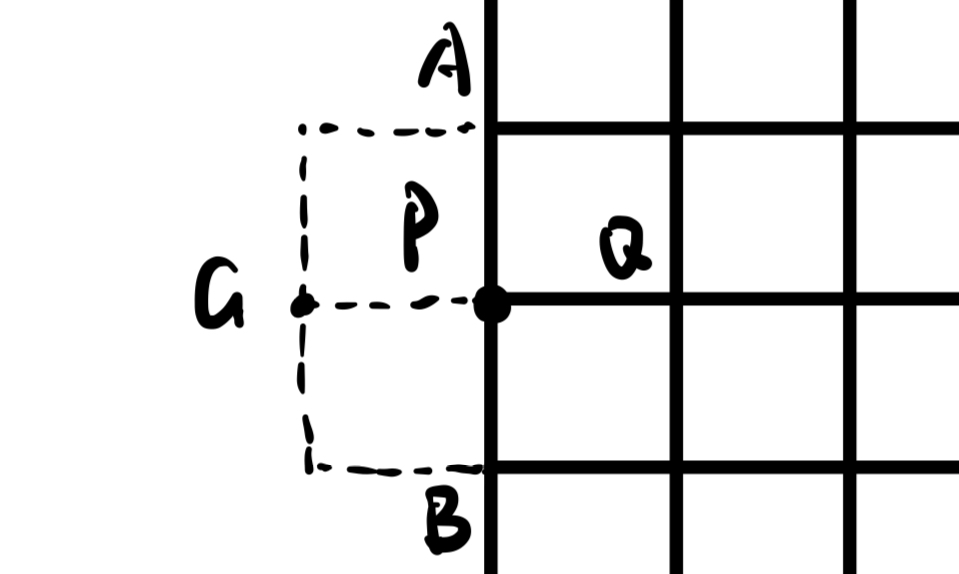
\includegraphics[width=0.4\linewidth]{discrete3.PNG}
        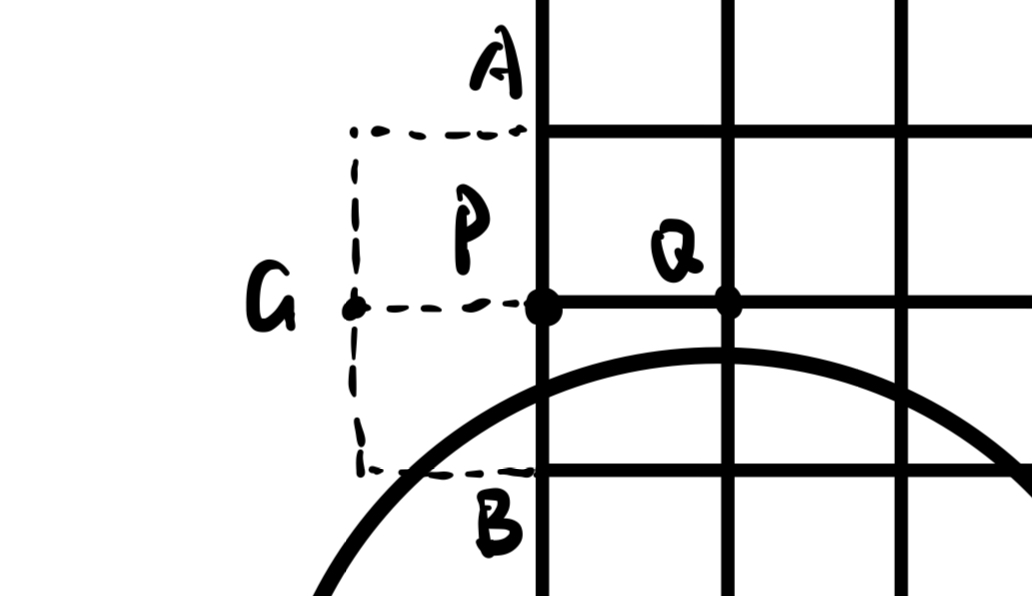
\includegraphics[width=0.4\linewidth]{discrete4.PNG}
    \end{figure}

    参照上边的过程其他方向的边界可以得到类似的差分格式,同一维的离散相同,这里是二阶精度的
\end{itemize}

\newpage

\subsection{2-D Gird Function Norm}
为了对结果误差进行分析我们需要将讲义中Gird Function Norm推广至二维

从一维的定义可以看出Gird Function 的 $L_q\ Norm: \left( h\sum_i |g_i|^q \right)^{\frac{1}{q}}$ 

其实是与function $L_q\ Norm:\left( \int |f|^qdx\right)^{\frac{1}{q}}$相一致的


那么对于二维的grid function参照二元函数的情形$L_q\ Norm:\left( \int |f|^qdxdy\right)^{\frac{1}{q}}$
$$L_q Norm(2D):\left( h^2\sum_i \sum_j |g_{ij}|^q \right)^{\frac{1}{q}}$$
\section{数值实验}
\subsection{概述}
\begin{itemize}
    \item 根据理论差分格式编写程序
    \item 在Regular和Irregular区域上以及组合不同的边界条件求解如下三个方程
    $$
    \begin{cases}
        -\Delta u(x,y) = (\sin(x)-\cos^2(x)-1)e^{y+\sin(x)} \\
        u(x,y)|_{\Gamma} = e^{y+\sin(x)}\\
        \frac{\partial u}{\partial n}|_{\Gamma} = \mathbf{n}\cdot \nabla e^{y+\sin(x)} 
    \end{cases}
    $$
    $$
    \begin{cases}
        -\Delta u(x,y) = 2\pi^2\sin(\pi x)\sin(\pi y) \\
        u(x,y)|_{\Gamma} = \sin(\pi x)\sin(\pi y)\\
        \frac{\partial u}{\partial n}|_{\Gamma} = \mathbf{n}\cdot \nabla \sin(\pi x)\sin(\pi y) 
    \end{cases}
    $$
    $$
    \begin{cases}
        -\Delta u(x,y) = -6(x+y) \\
        u(x,y)|_{\Gamma} = x^3+y^3\\
        \frac{\partial u}{\partial n}|_{\Gamma} = \mathbf{n}\cdot \nabla (x^3+y^3) 
    \end{cases}
    $$
    \item Irrgular区域的圆的参数设置为圆心$(0.1,0.1)$,半径$r=0.3$,如下图红色区域所示
    \begin{figure}[h]
        \centering
        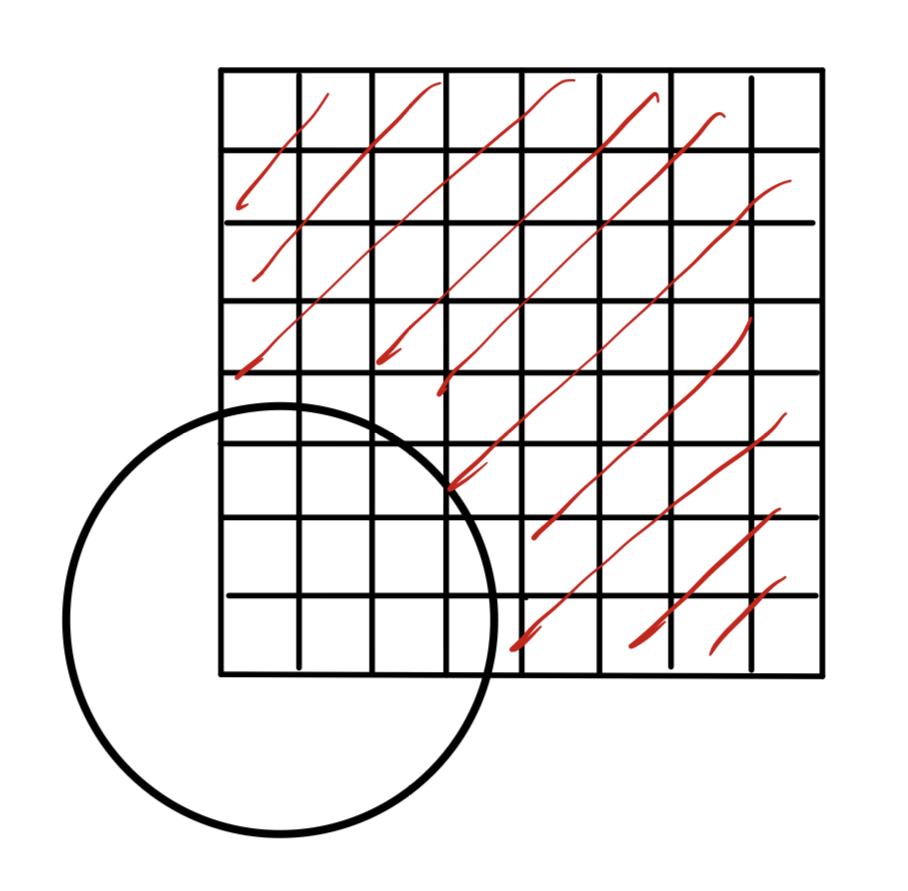
\includegraphics[width=0.5\linewidth]{irregularDomain.jpg}
    \end{figure}
    \item 边界条件取了如下九种:Regular,纯Dirichlet,纯Nuemann,有一条边界为Nuemann,两条相同条件的边界对边,两条相同条件的边界相邻;Irregular, 为了简化测试,我们将整个方形边框看成一整个边界,则边界条件为全Dirichlet,全Nuemann,方Dirichlet圆Nuemann,方Nuemann圆Dirichlet。
    \item 求解将结果输出到文件,文件编号说明,test1/2/3对应三个不同方程、n=x为网格大小、IRD/RD(Irregualr Domain/Regular Domain)、后面的数字为边界条件(0为Dirichlet,1为Nuemann,按顺序为下右上左圆)、E/U/ErrorNorm(误差绝对值/数值解/误差范数,误差范数按列存储从左到右为$L_1,L_2,L_{\infty}$)。例,test1n=64RD0000E为在$n=64$的网格上以纯Dirichlet条件求解方程的误差绝对值
    \item 将误差以热力图的形式绘制,纯黑色部分为边界,如下图所示,对于同一个问题在不同粗细的网格上求解,其误差在空间上的分布基本相同,为节省篇幅所以后面的实验结果将只放出最细网格的热力图
    \begin{figure}[h]
        \centering
        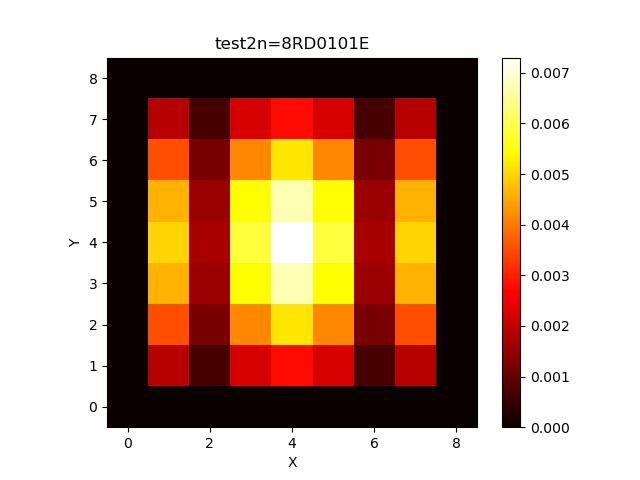
\includegraphics[width=0.4\linewidth]{test2n=8RD0101E.jpg}
        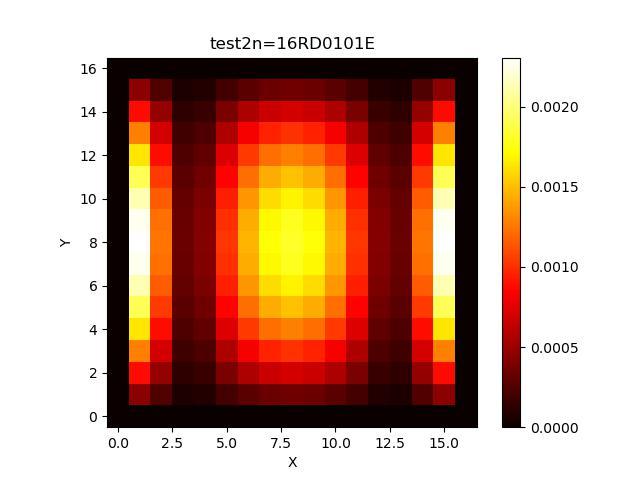
\includegraphics[width=0.4\linewidth]{test2n=16RD0101E.jpg}\\
        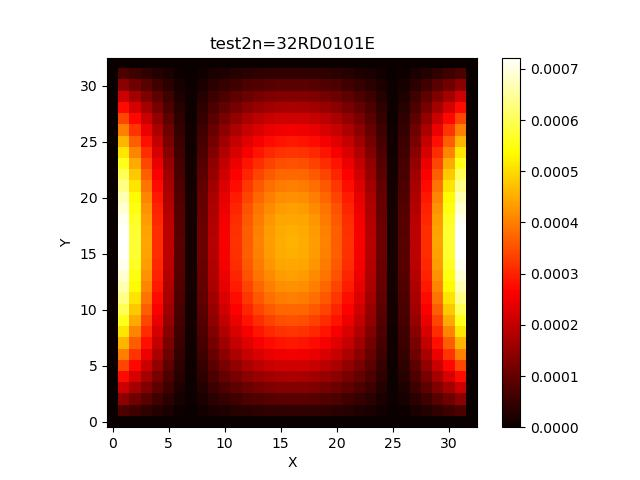
\includegraphics[width=0.4\linewidth]{test2n=32RD0101E.jpg}
        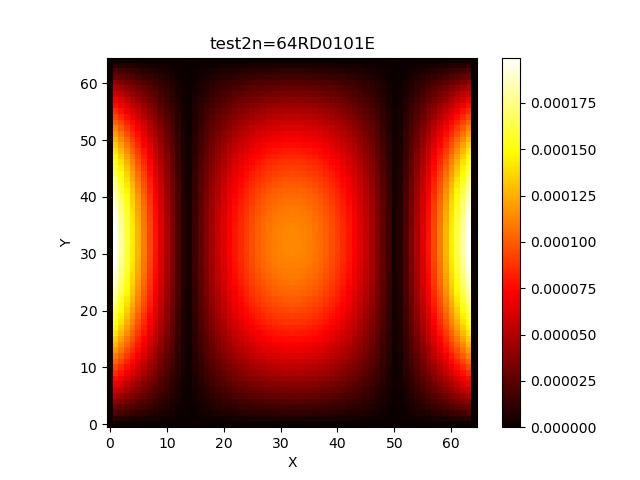
\includegraphics[width=0.4\linewidth]{test2n=64RD0101E.jpg}
    \end{figure}
    \item 将误差的网格范数$\left \| E \right \| = O(h^{\alpha})$两边取对数得$$\log\left \| E \right \| = \alpha \log O(h)$$
        绘制图像判断斜率即可判断算法的收敛阶
\end{itemize}

\newpage
\subsection{实验结果}
\subsubsection{$u(x,y)=e^{y+\sin(x)}$}
真实值:
\begin{figure}[h]
    \centering
    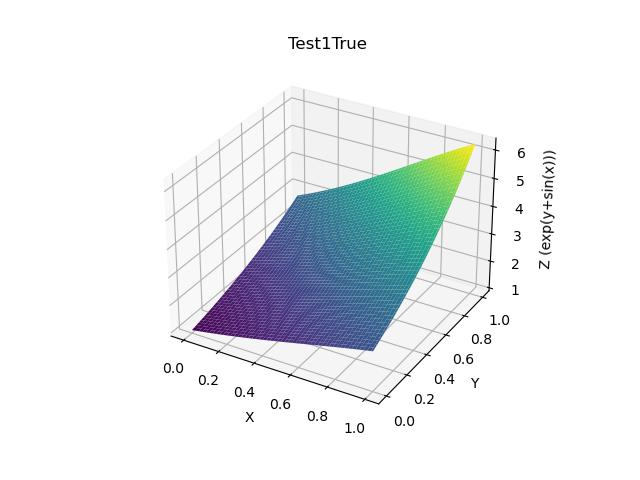
\includegraphics[width=0.7\linewidth]{Test1True.jpg}
\end{figure}
\begin{itemize}
    \item Regular 纯Dirichlet边界
    \begin{figure}[h]
        \centering
        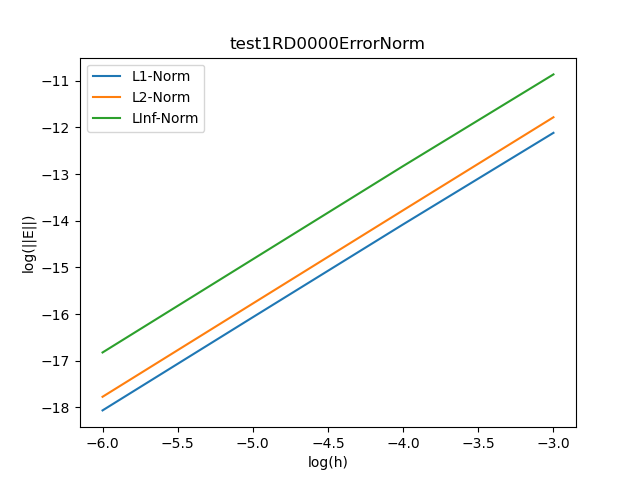
\includegraphics[width=0.35\linewidth]{test1RD0000ErrorNormjpg.png}
        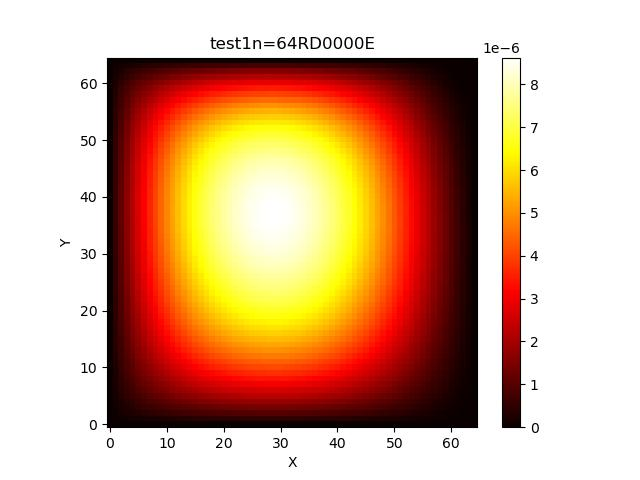
\includegraphics[width=0.35\linewidth]{test1n=64RD0000E.jpg}
    \end{figure}

    从图像斜率可以看出收敛阶大约为2
    \item Regular 左边界为Nuemann条件其余为Dirichlet
    \begin{figure}[h]
        \centering
        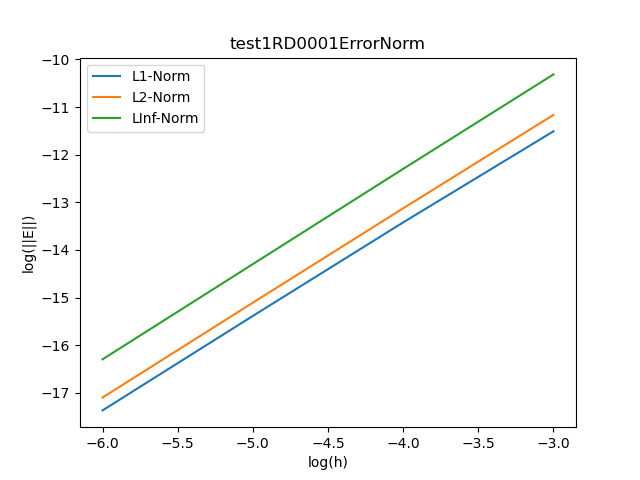
\includegraphics[width=0.35\linewidth]{test1RD0001ErrorNormjpg.png}
        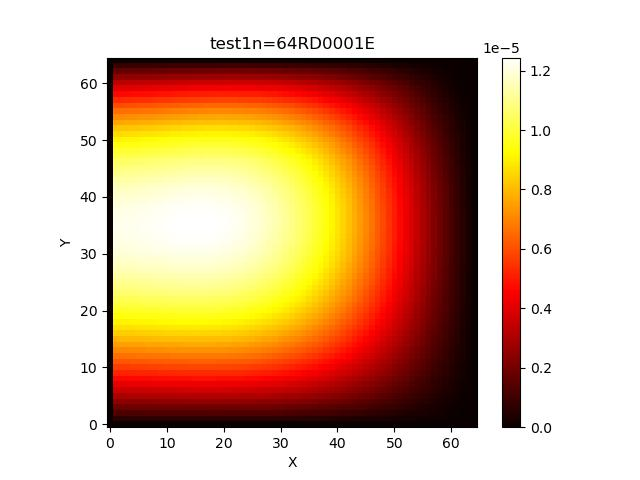
\includegraphics[width=0.35\linewidth]{test1n=64RD0001E.jpg}
    \end{figure}

    从图像斜率可以看出收敛阶大约为2
    \newpage
    \item Regular 上下为Dirichlet、左右为Nuemann
    \begin{figure}[h]
        \centering
        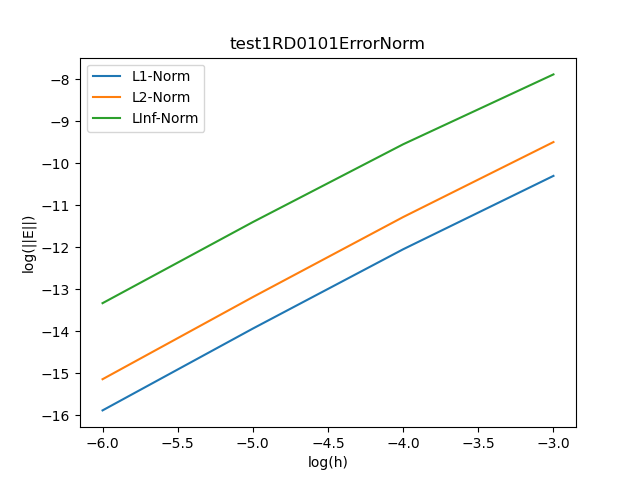
\includegraphics[width=0.35\linewidth]{test1RD0101ErrorNormjpg.png}
        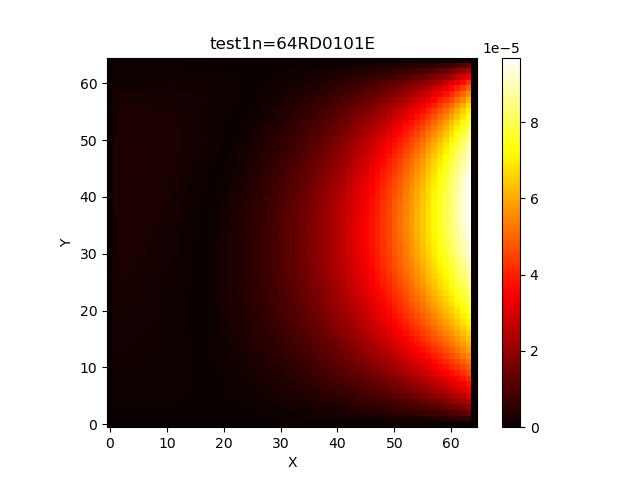
\includegraphics[width=0.35\linewidth]{test1n=64RD0101E.jpg}
    \end{figure}

    从图像斜率可以看出收敛阶大约为2
    \item Regular 下右为Dirichlet、上左为Nuemann
    \begin{figure}[h]
        \centering
        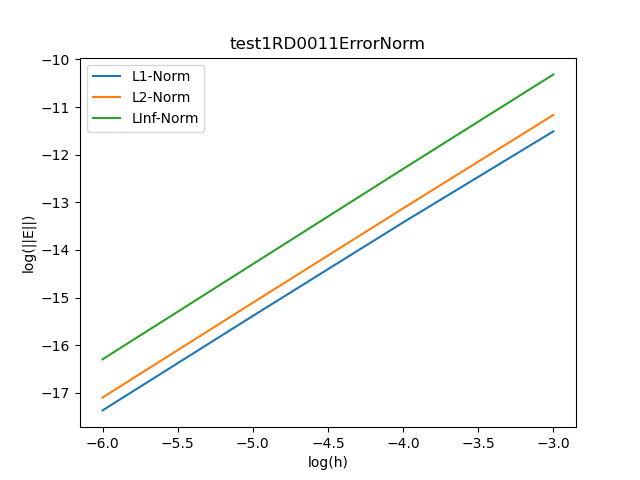
\includegraphics[width=0.35\linewidth]{test1RD0011ErrorNormjpg.png}
        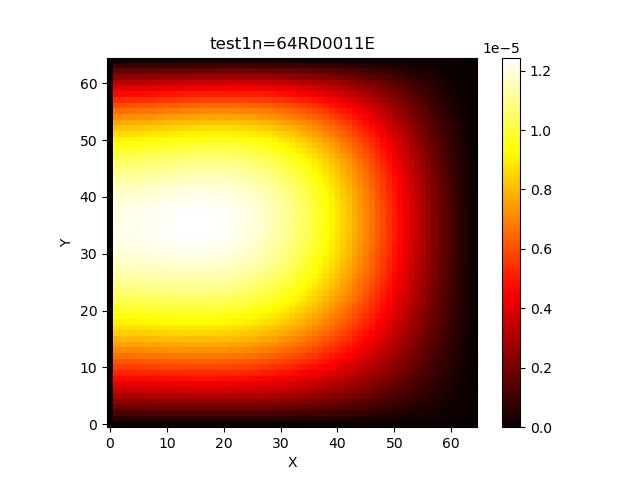
\includegraphics[width=0.35\linewidth]{test1n=64RD0011E.jpg}
    \end{figure}

    从图像斜率可以看出收敛阶大约为2
    \item Regular 纯Nuemann
    \begin{figure}[h]
        \centering
        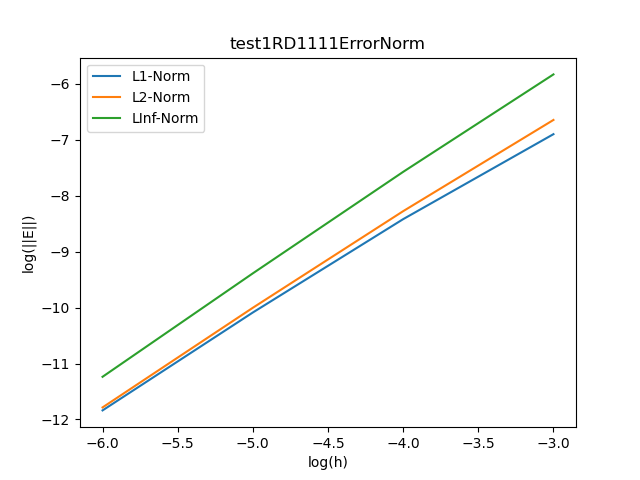
\includegraphics[width=0.35\linewidth]{test1RD1111ErrorNormjpg.png}
        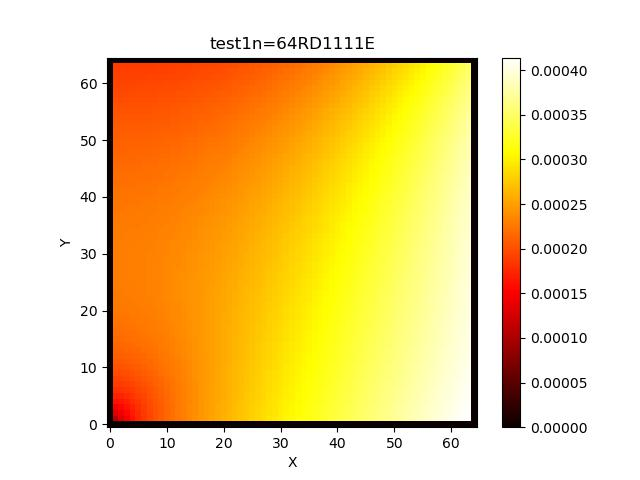
\includegraphics[width=0.35\linewidth]{test1n=64RD1111E.jpg}
    \end{figure}

    从图像斜率可以看出收敛阶大约为2
    \newpage
    \item Irregular 纯Dirichlet
    \begin{figure}[h]
        \centering
        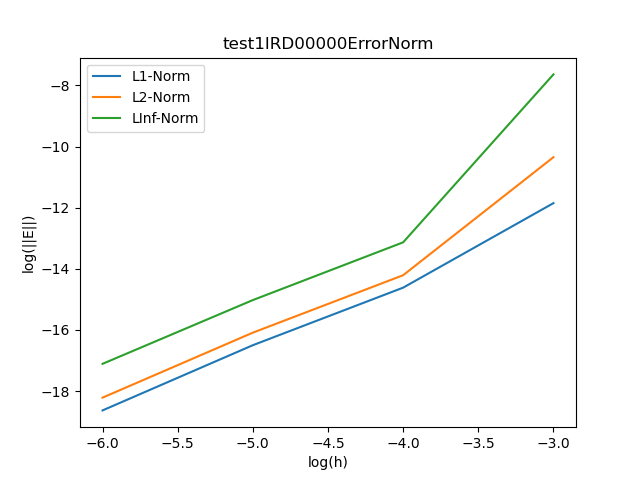
\includegraphics[width=0.35\linewidth]{test1IRD00000ErrorNormjpg.png}
        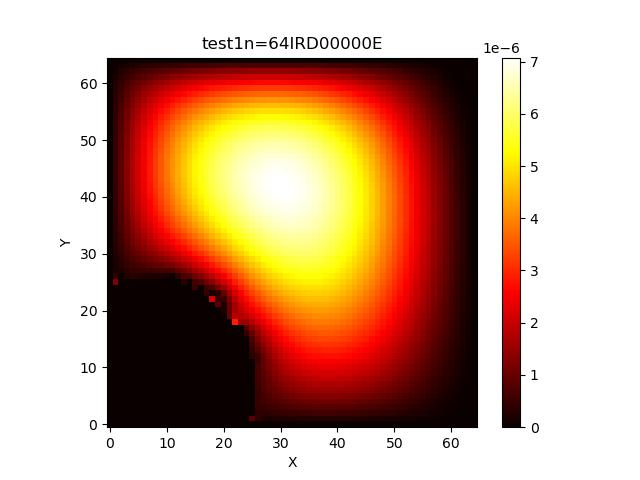
\includegraphics[width=0.35\linewidth]{test1n=64IRD00000E.jpg}
    \end{figure}

    从图像斜率可以看出收敛阶大约为2
    \item Irregular 方形边界为Dirichlet、圆为Nuemann
    \begin{figure}[h]
        \centering
        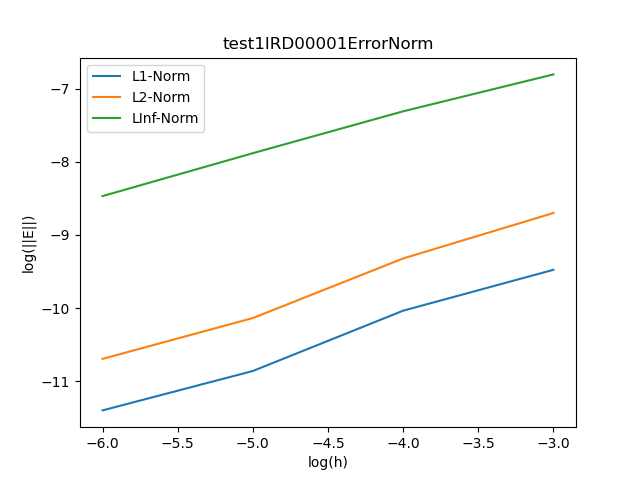
\includegraphics[width=0.35\linewidth]{test1IRD00001ErrorNormjpg.png}
        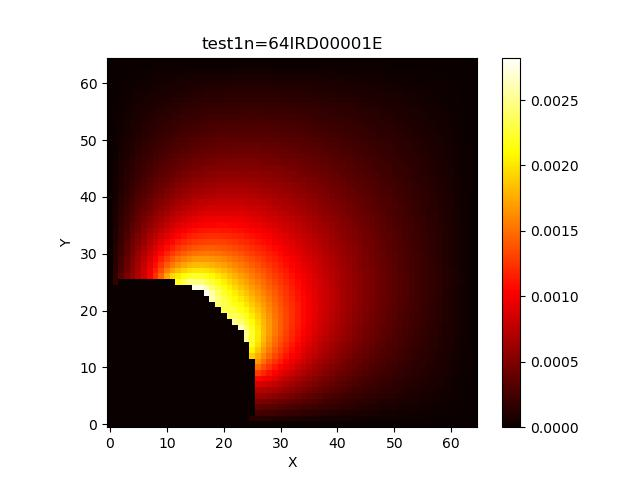
\includegraphics[width=0.35\linewidth]{test1n=64IRD00001E.jpg}
    \end{figure}

    从图像斜率可以看出收敛阶大约为1
    \item Irregular 方形边界为Nuemann、圆为Dirichlet
    \begin{figure}[h]
        \centering
        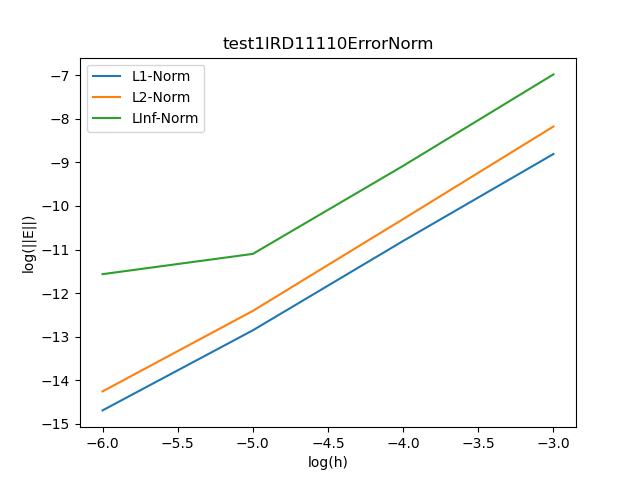
\includegraphics[width=0.35\linewidth]{test1IRD11110ErrorNormjpg.png}
        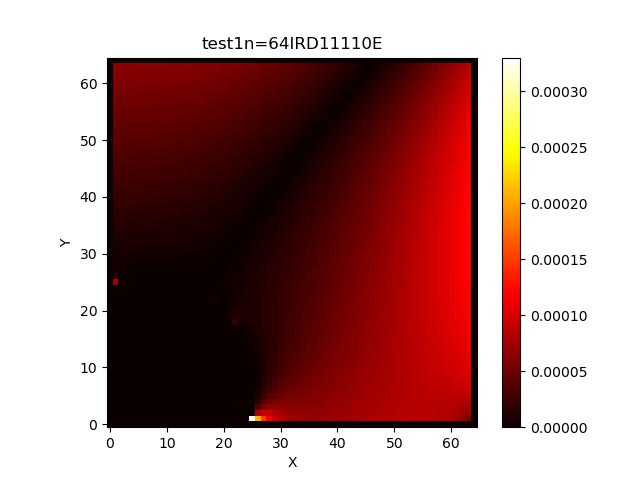
\includegraphics[width=0.35\linewidth]{test1n=64IRD11110E.jpg}
    \end{figure}

    从图像斜率可以看出收敛阶大约为2
    \newpage
    \item Irregular 纯Nuemann
    \begin{figure}[h]
        \centering
        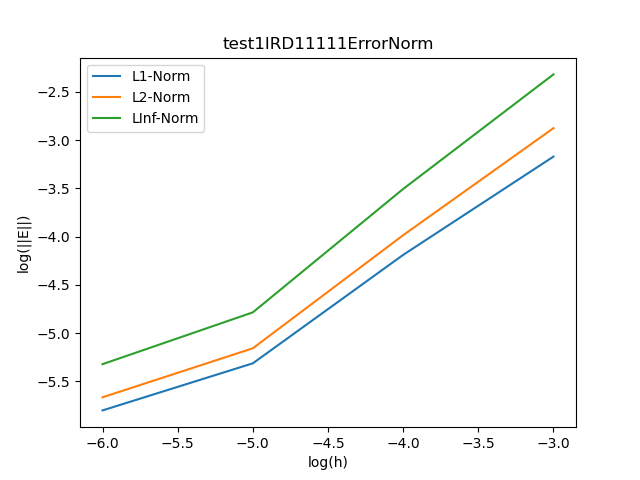
\includegraphics[width=0.35\linewidth]{test1IRD11111ErrorNormjpg.png}
        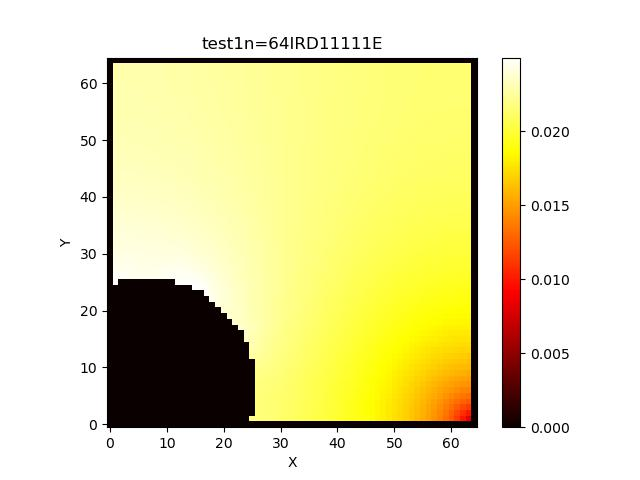
\includegraphics[width=0.35\linewidth]{test1n=64IRD11111E.jpg}
    \end{figure}

    从图像斜率可以看出收敛阶大约为1
\end{itemize}

\subsubsection{$u(x,y)=\sin(\pi x)\sin(\pi y)$}
真实值:
\begin{figure}[h]
    \centering
    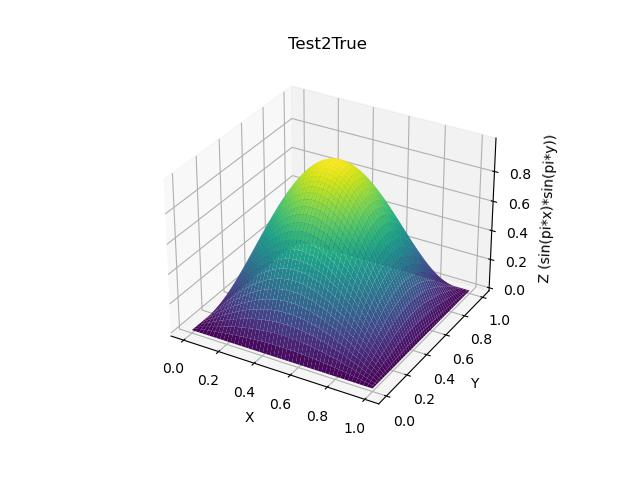
\includegraphics[width=0.7\linewidth]{Test2True.jpg}
\end{figure}
\begin{itemize}
    \item Regular 纯Dirichlet边界
    \begin{figure}[h]
        \centering
        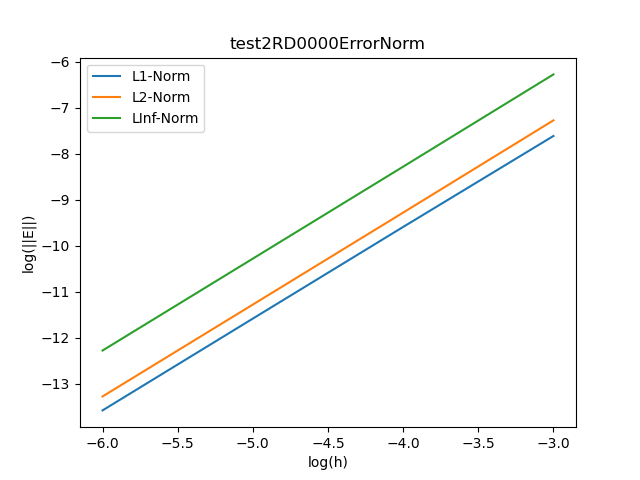
\includegraphics[width=0.35\linewidth]{test2RD0000ErrorNormjpg.png}
        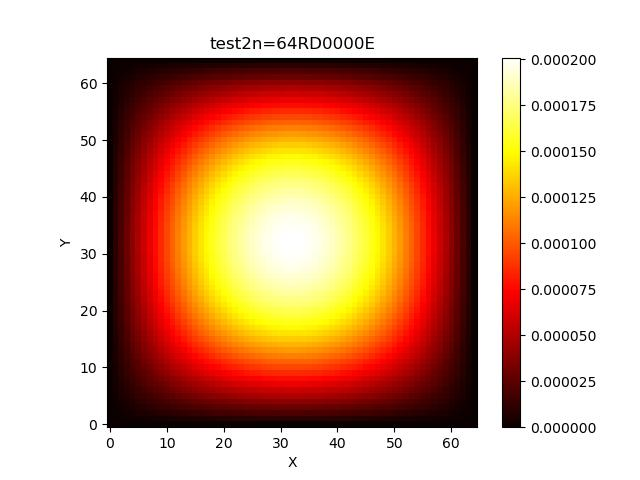
\includegraphics[width=0.35\linewidth]{test2n=64RD0000E.jpg}
    \end{figure}
    
    从图像斜率可以看出收敛阶大约为2
    \newpage
    \item Regular 左边界为Nuemann条件其余为Dirichlet
    \begin{figure}[h]
        \centering
        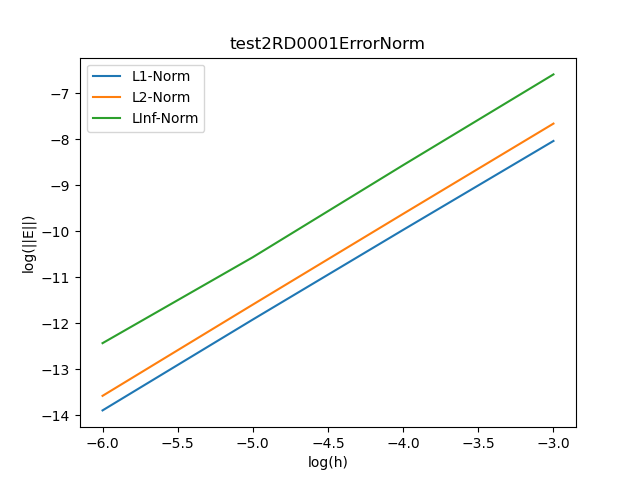
\includegraphics[width=0.35\linewidth]{test2RD0001ErrorNormjpg.png}
        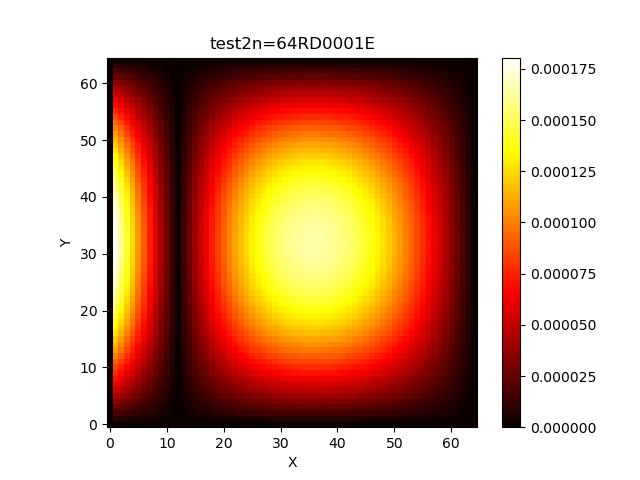
\includegraphics[width=0.35\linewidth]{test2n=64RD0001E.jpg}
    \end{figure}

    从图像斜率可以看出收敛阶大约为2
    
    \item Regular 上下为Dirichlet、左右为Nuemann
    \begin{figure}[h]
        \centering
        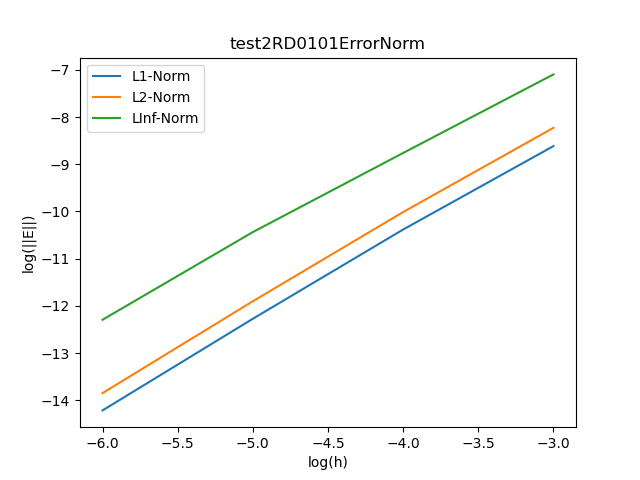
\includegraphics[width=0.35\linewidth]{test2RD0101ErrorNormjpg.png}
        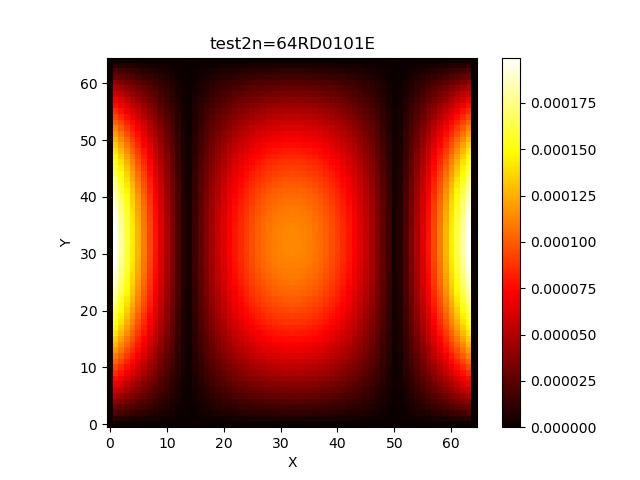
\includegraphics[width=0.35\linewidth]{test2n=64RD0101E.jpg}
    \end{figure}

    从图像斜率可以看出收敛阶大约为2
    \item Regular 下右为Dirichlet、上左为Nuemann
    \begin{figure}[h]
        \centering
        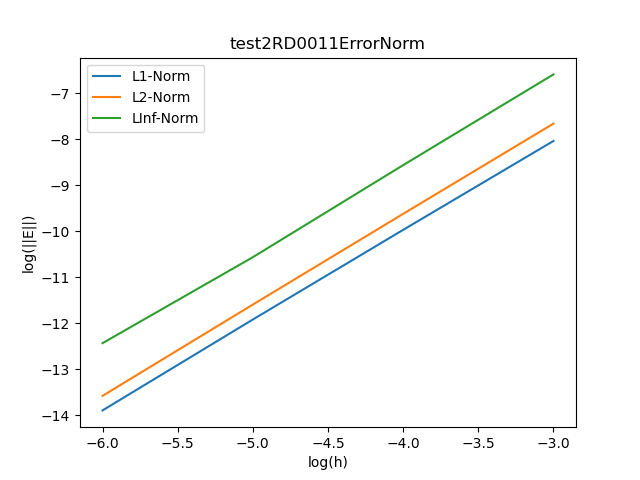
\includegraphics[width=0.35\linewidth]{test2RD0011ErrorNormjpg.png}
        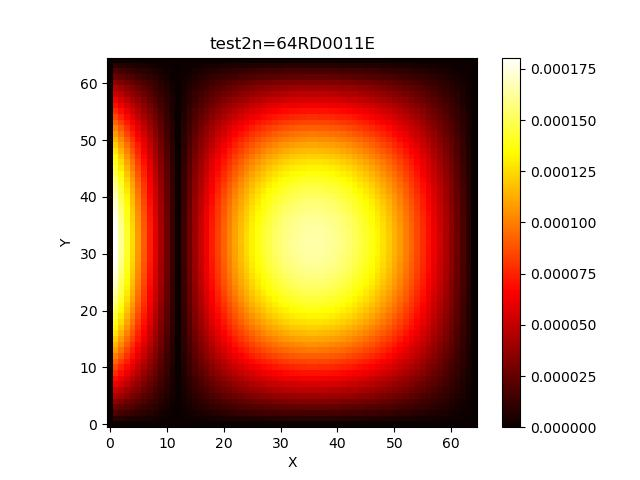
\includegraphics[width=0.35\linewidth]{test2n=64RD0011E.jpg}
    \end{figure}
    
    从图像斜率可以看出收敛阶大约为2
    \newpage
    \item Regular 纯Nuemann
    \begin{figure}[h]
        \centering
        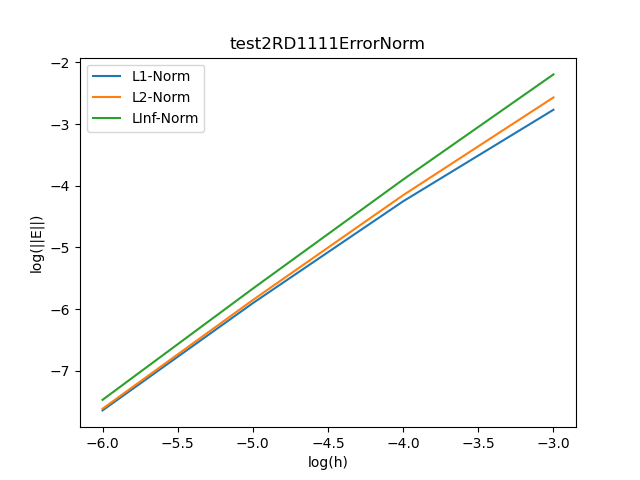
\includegraphics[width=0.35\linewidth]{test2RD1111ErrorNormjpg.png}
        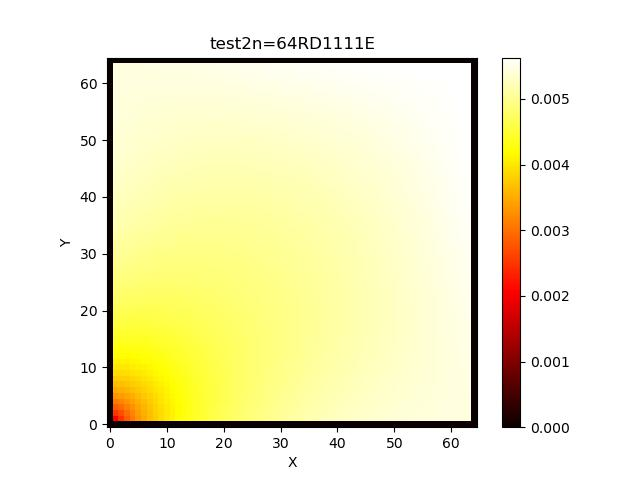
\includegraphics[width=0.35\linewidth]{test2n=64RD1111E.jpg}
    \end{figure}

    从图像斜率可以看出收敛阶大约为2
    \item Irregular 纯Dirichlet
    \begin{figure}[h]
        \centering
        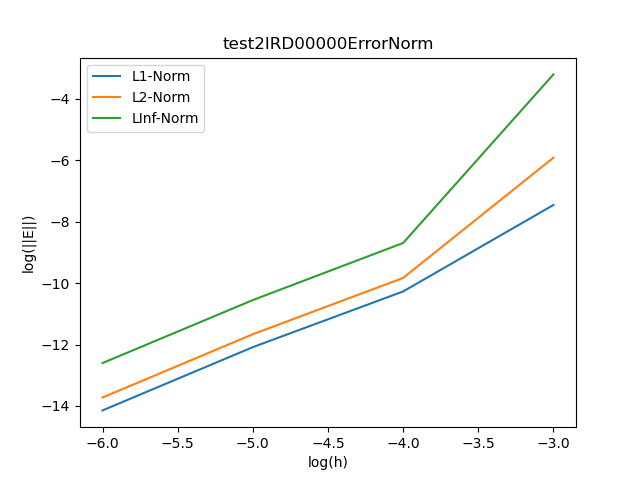
\includegraphics[width=0.35\linewidth]{test2IRD00000ErrorNormjpg.png}
        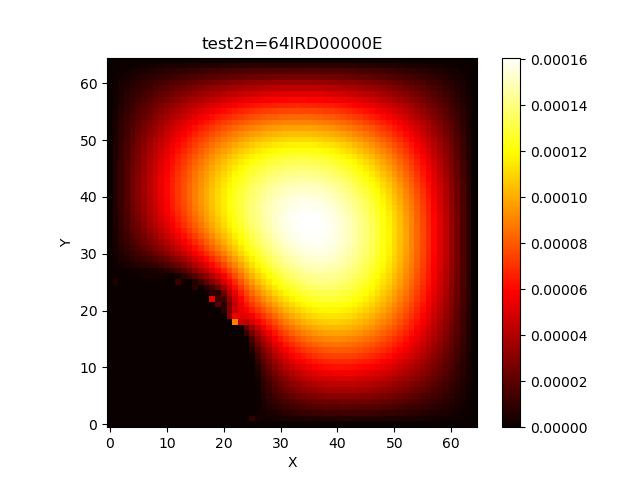
\includegraphics[width=0.35\linewidth]{test2n=64IRD00000E.jpg}
    \end{figure}

    从图像斜率可以看出收敛阶大约为2
    \item Irregular 方形边界为Dirichlet、圆为Nuemann
    \begin{figure}[h]
        \centering
        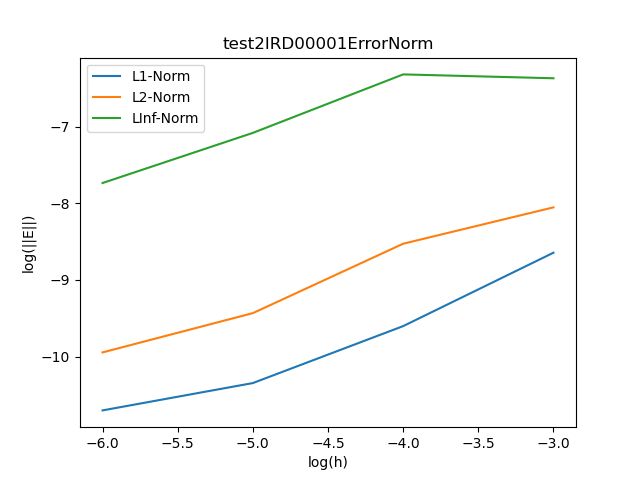
\includegraphics[width=0.35\linewidth]{test2IRD00001ErrorNormjpg.png}
        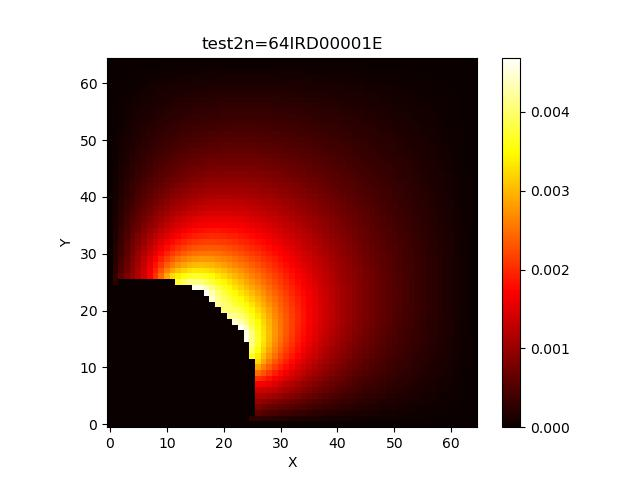
\includegraphics[width=0.35\linewidth]{test2n=64IRD00001E.jpg}
    \end{figure}

    从图像斜率可以看出收敛阶大约为1
    \newpage
    \item Irregular 方形边界为Nuemann、圆为Dirichlet
    \begin{figure}[h]
        \centering
        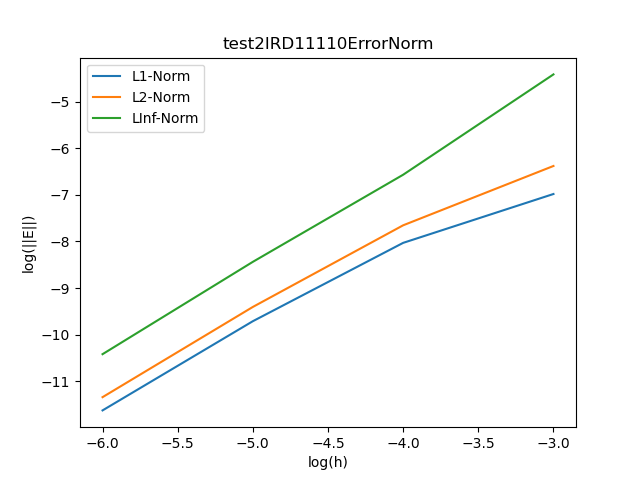
\includegraphics[width=0.35\linewidth]{test2IRD11110ErrorNormjpg.png}
        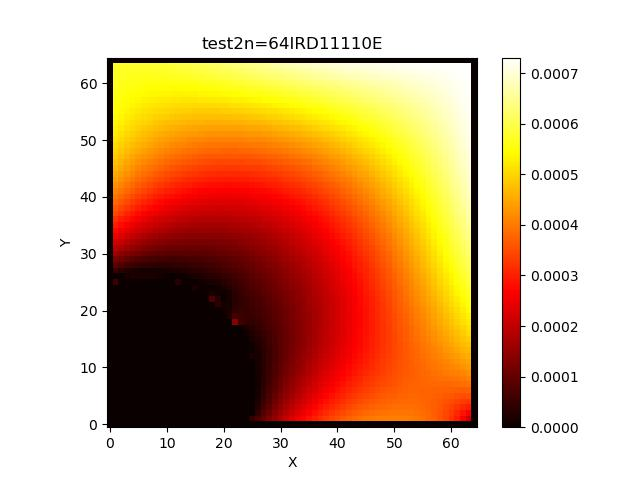
\includegraphics[width=0.35\linewidth]{test2n=64IRD11110E.jpg}
    \end{figure}

    从图像斜率可以看出收敛阶大约为2
    \item Irregular 纯Nuemann
    \begin{figure}[h]
        \centering
        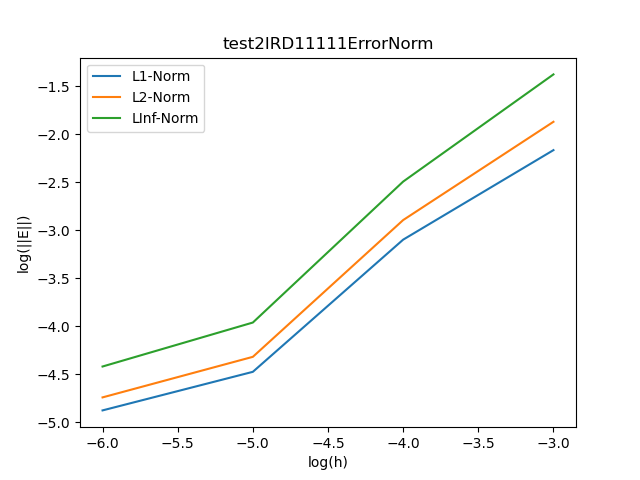
\includegraphics[width=0.35\linewidth]{test2IRD11111ErrorNormjpg.png}
        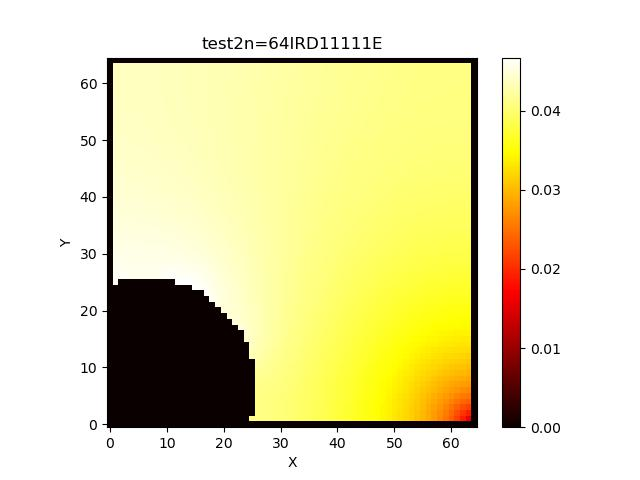
\includegraphics[width=0.35\linewidth]{test2n=64IRD11111E.jpg}
    \end{figure}

    从图像斜率可以看出收敛阶大约为1
\end{itemize}

\subsubsection{$u(x,y)=x^3+y^3$}
真实值:
\begin{figure}[h]
    \centering
    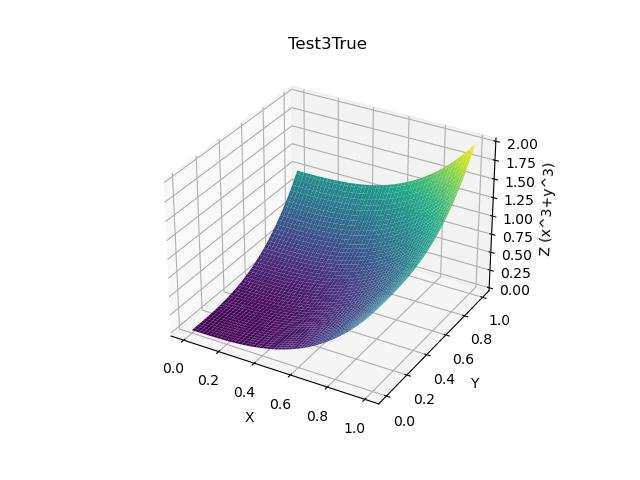
\includegraphics[width=0.7\linewidth]{Test3True.jpg}
\end{figure}
\begin{itemize}
    \newpage
    \item Regular 纯Dirichlet边界
    \begin{figure}[h]
        \centering
        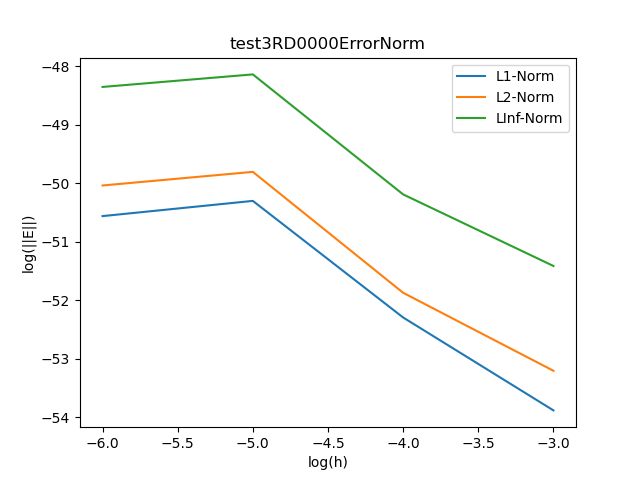
\includegraphics[width=0.35\linewidth]{test3RD0000ErrorNormjpg.png}
        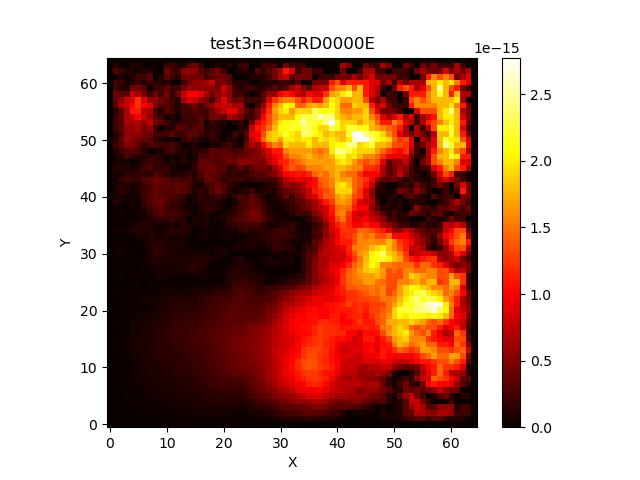
\includegraphics[width=0.35\linewidth]{test3n=64RD0000E.jpg}
    \end{figure}
    
    虽然图像不符合正常情况,但是从数值上来看其误差已经非常小,可以认为是数值精度的影响,并且从热力图上也可以看出误差分布在其本来的误差分布叠加了一个随机的误差分布,因此也认为达到了2阶的收敛阶
    \item Regular 左边界为Nuemann条件其余为Dirichlet
    \begin{figure}[h]
        \centering
        \includegraphics[width=0.35\linewidth]{test3RD0001ErrorNormjpg.png}
        \includegraphics[width=0.35\linewidth]{test3n=64RD0001E.jpg}
    \end{figure}

    从图像斜率可以看出收敛阶大约为2
    
    \item Regular 上下为Dirichlet、左右为Nuemann
    \begin{figure}[h]
        \centering
        \includegraphics[width=0.35\linewidth]{test3RD0101ErrorNormjpg.png}
        \includegraphics[width=0.35\linewidth]{test3n=64RD0101E.jpg}
    \end{figure}

    从图像斜率可以看出收敛阶大约为2
    \newpage
    \item Regular 下右为Dirichlet、上左为Nuemann
    \begin{figure}[h]
        \centering
        \includegraphics[width=0.35\linewidth]{test3RD0011ErrorNormjpg.png}
        \includegraphics[width=0.35\linewidth]{test3n=64RD0011E.jpg}
    \end{figure}
    
    从图像斜率可以看出收敛阶大约为2
    \item Regular 纯Nuemann
    \begin{figure}[h]
        \centering
        \includegraphics[width=0.35\linewidth]{test3RD1111ErrorNormjpg.png}
        \includegraphics[width=0.35\linewidth]{test3n=64RD1111E.jpg}
    \end{figure}

    从图像斜率可以看出收敛阶大约为2
    \item Irregular 纯Dirichlet
    \begin{figure}[h]
        \centering
        \includegraphics[width=0.35\linewidth]{test3IRD00000ErrorNormjpg.png}
        \includegraphics[width=0.35\linewidth]{test3n=64IRD00000E.jpg}
    \end{figure}

    从图像斜率可以看出收敛阶大约为2
    \newpage
    \item Irregular 方形边界为Dirichlet、圆为Nuemann
    \begin{figure}[h]
        \centering
        \includegraphics[width=0.35\linewidth]{test3IRD00001ErrorNormjpg.png}
        \includegraphics[width=0.35\linewidth]{test3n=64IRD00001E.jpg}
    \end{figure}

    从图像斜率可以看出收敛阶大约为1
    \item Irregular 方形边界为Nuemann、圆为Dirichlet
    \begin{figure}[h]
        \centering
        \includegraphics[width=0.35\linewidth]{test3IRD11110ErrorNormjpg.png}
        \includegraphics[width=0.35\linewidth]{test3n=64IRD11110E.jpg}
    \end{figure}

    从图像斜率可以看出收敛阶大约为2
    \item Irregular 纯Nuemann
    \begin{figure}[h]
        \centering
        \includegraphics[width=0.35\linewidth]{test3IRD11111ErrorNormjpg.png}
        \includegraphics[width=0.35\linewidth]{test3n=64IRD11111E.jpg}
    \end{figure}

    图像斜率应该可以算作收敛阶为1
\end{itemize}

\subsection{总结分析}
从上面的三组测试样例可以看出,除了圆形边界上为Nuemann边界条件的情况,其他情况均达到了二阶的收敛率,验证了只有一阶精度的Dirichlet条件下的Irregular point并不会影响到整体的二阶收敛率。
此外,从误差分布的热力图可以看出,Irregular边界以及Nuemann边界附近的误差较大,而Dirichlet边界附近的误差相对较小,且Nuemann条件的影响远大于Irregular边界的影响。

\end{document}